\documentclass[11pt]{article}

\usepackage[margin=1.6cm]{geometry}
\usepackage{amsmath,amssymb,amsthm}
\usepackage[hidelinks]{hyperref}
\usepackage[most]{tcolorbox}
\usepackage[]{cancel}
\usepackage{tikz-feynman}
\usepackage{slashed}
\tikzfeynmanset{compat=1.1.0}
\newenvironment{solution}[1][]{\begin{proof}[\textbf{Solution}]}{\end{proof}}
% --- Rounded box style for each problem (whole statement) ---
\tcbset{
    problem/.style={
        enhanced,
        boxrule=0.7pt,
        arc=3mm,
        left=3mm,right=3mm,top=2mm,bottom=2mm,
        colback=white,
        colframe=black,
        before skip=10pt,
        after skip=6pt,
    }
}

\begin{document}
\begin{center}
    {\LARGE \textbf{Solution Manual of Problem Set 15} \par}
    \vspace{1em}
    {\large Bufan Zheng\\ \href{mailto:bufan@g.ecc.u-tokyo.ac.jp}{\texttt{bufan@g.ecc.u-tokyo.ac.jp}} \par}
\end{center}


\begin{tcolorbox}[problem]
\textbf{1.} Define ``soft divergence'' and ``collinear divergence'' in terms of regions of loop or phase-space integration.
\end{tcolorbox}
\begin{solution}[15.1]
	Soft singularities occur when the momentum of a massless particle goes to zero. Feynman diagrams of the form
	\[
	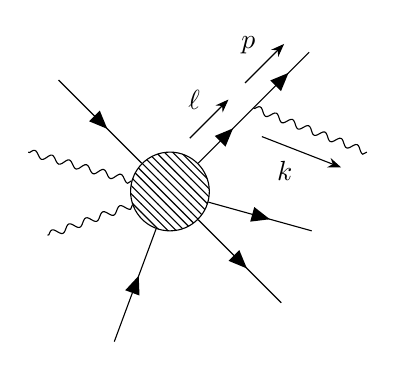
\begin{tikzpicture}[baseline=(current bounding box.center)]
		\begin{feynman}
			% 1. 定义中心标准 blob
			% 可以通过 minimum size 稍微调整它的大小
			\vertex [blob, minimum size=1cm] (c) {};
			
			% 2. 定义周围的顶点位置（手动指定以模拟原图的随意感）
			% 左侧入射
			\vertex [above left=2cm of c] (i1);
			\vertex [left=1.8cm of c, yshift=0.5cm] (i2);
			\vertex [below left=2.2cm of c, yshift=1cm] (i3);
			\vertex [below left=1cm of c,yshift=-1.2cm, rotate=-20] (i4);
			
			% 右侧出射
			% 关键的带动量 k 的光子顶点位置
			\vertex [above right=2.5cm of c] (o_k); 
			\vertex [above right=1.5cm of c] (o_f); 
			\vertex [right=2.5cm of c,yshift=0.5cm] (o_f2); 
			% 其他出射粒子
			\vertex [below right=2cm of c] (o2);
			\vertex [right=1.8cm of c, yshift=-0.5cm] (o3);
			
			% 3. 绘制连接线 (使用 \diagram* 手动模式)
			\diagram* {
				% 入射粒子 (混合直线和波浪线)
				(i1) -- [fermion] (c),
				(i2) -- [photon] (c),
				(i3) -- [photon] (c),
				(i4) -- [fermion] (c),
				
				% 关键：带有动量 k 的出射光子
				% momentum 选项会自动添加箭头和标签
				(c) -- [fermion, momentum=$\ell$] (o_f),
				(o_f) -- [fermion,momentum=$p$](o_k),
				(o_f) -- [photon, momentum'=$k$](o_f2),
				
				% 其他出射粒子
				(c) -- [fermion] (o2),
				(c) -- [fermion] (o3),
			};
		\end{feynman}
	\end{tikzpicture}
	\]
	develop a singularity in this limit because the propagator, goes on-shell, i.e. $\ell=k+p\to p$.
	
	Another type of amplitude singularity arises when two external momenta become collinear. Diagrams in which the two external legs attach to a common 3-vertex are then divergent because the internal propagator goes on-shell. Still using the diagram above as an example, we assume the electron is massless. When the emitted photon momentum is parallel to the outgoing electron momentum, namely \(k \propto p\), we clearly have \(\ell \propto k \propto p\). Since \(k^2 = 0\), it follows that the propagator satisfies \(\ell^2 = 0\), meaning the internal propagator goes on shell, which leads to a divergence.
\end{solution}
\begin{tcolorbox}[problem]
\textbf{2.} Show by power counting in $D$ dimensions that the phase space measure for emission of a soft massless boson behaves like $d^Dk\,\delta(k^2)\theta(k^0)\sim k^{D-3}dk$. For which $D$ does $$\int_0 dk\,\frac{k^{D-3}}{k}$$ diverge? (soft factor $\sim 1/k$)
\end{tcolorbox}
\begin{solution}[15.2]
	The phase measure for massless boson behaves like:
	\[
	\begin{aligned}
	d^Dk\,\delta(k^2)\,\theta(k^0)
	&= dk^0\,d^{D-1}\mathbf{k}\,\delta\!\big((k^0)^2-\mathbf{k}^2\big)\,\theta(k^0)
	= dk^0\,d^{D-1}\mathbf{k}\,\frac{\delta(k^0-|\mathbf{k}|)}{2|\mathbf{k}|}\\
	&= \frac{d^{D-1}\mathbf{k}}{2|\mathbf{k}|}
	= \frac{k^{D-2}dk\,d\Omega_{D-2}}{2k}
	\sim k^{D-3}\,dk .
	\end{aligned}
	\]
	Next, consider the soft limit, we encounter the following integral:
	\[
	\int_0dk\frac{k^{D-3}}{k}\sim k^{D-3}
	\]
	It is clear the divergence appear when $D-3\leq 0$. So \textbf{MY FINAL ANSWER IS}:
	\[
	\boxed{
	D\leq 3
	}
	\]
\end{solution}
\begin{tcolorbox}[problem]
\textbf{3.} For massless charged particles in $D=4$, explain why collinear divergences appear but are absent if the charged particle has a nonzero mass.
\end{tcolorbox}
\begin{solution}[15.3]
	From the discussion in Problem~1, we can see that regardless of whether the electron is massless, when the momentum of the radiated photon approaches zero, the internal electron propagator goes on shell, i.e.\ \(\ell^2 = m^2\). However, when we consider the collinear limit, we can only obtain \(\ell^2 \propto k^2 = 0\). Therefore, only when the electron is massless can we say that the propagator goes on shell and thus produces a divergence. If the electron is massive, the denominator of the propagator still receives a nonzero contribution of \(m^2\).
\end{solution}
\begin{tcolorbox}[problem]
\textbf{4.} Derive the eikonal factor for soft photon emission off an external leg, $\sim e\,\frac{p\cdot\epsilon}{p\cdot k}$. Explain why it is universal.
\end{tcolorbox}
\begin{solution}[15.4]
	Consider the following diagram:
		\[
	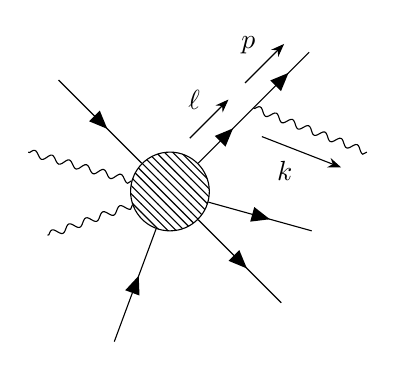
\begin{tikzpicture}[baseline=(current bounding box.center)]
		\begin{feynman}
			% 1. 定义中心标准 blob
			% 可以通过 minimum size 稍微调整它的大小
			\vertex [blob, minimum size=1cm] (c) {};
			
			% 2. 定义周围的顶点位置（手动指定以模拟原图的随意感）
			% 左侧入射
			\vertex [above left=2cm of c] (i1);
			\vertex [left=1.8cm of c, yshift=0.5cm] (i2);
			\vertex [below left=2.2cm of c, yshift=1cm] (i3);
			\vertex [below left=1cm of c,yshift=-1.2cm, rotate=-20] (i4);
			
			% 右侧出射
			% 关键的带动量 k 的光子顶点位置
			\vertex [above right=2.5cm of c] (o_k); 
			\vertex [above right=1.5cm of c] (o_f); 
			\vertex [right=2.5cm of c,yshift=0.5cm] (o_f2); 
			% 其他出射粒子
			\vertex [below right=2cm of c] (o2);
			\vertex [right=1.8cm of c, yshift=-0.5cm] (o3);
			
			% 3. 绘制连接线 (使用 \diagram* 手动模式)
			\diagram* {
				% 入射粒子 (混合直线和波浪线)
				(i1) -- [fermion] (c),
				(i2) -- [photon] (c),
				(i3) -- [photon] (c),
				(i4) -- [fermion] (c),
				
				% 关键：带有动量 k 的出射光子
				% momentum 选项会自动添加箭头和标签
				(c) -- [fermion, momentum=$\ell$] (o_f),
				(o_f) -- [fermion,momentum=$p$](o_k),
				(o_f) -- [photon, momentum'=$k$](o_f2),
				
				% 其他出射粒子
				(c) -- [fermion] (o2),
				(c) -- [fermion] (o3),
			};
		\end{feynman}
	\end{tikzpicture}
	\quad=\quad
	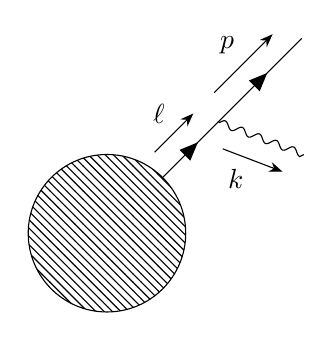
\begin{tikzpicture}[baseline=(current bounding box.center)]
		\begin{feynman}
			% 1. 定义中心标准 blob
			% 可以通过 minimum size 稍微调整它的大小
			\vertex [blob, minimum size=2cm] (c) {};
			
			% 2. 定义周围的顶点位置（手动指定以模拟原图的随意感）
			
			% 右侧出射
			% 关键的带动量 k 的光子顶点位置
			\vertex [above right=3.5cm of c] (o_k); 
			\vertex [above right=2cm of c] (o_f); 
			\vertex [right=2.5cm of c,yshift=1cm] (o_f2); 
			
			% 3. 绘制连接线 (使用 \diagram* 手动模式)
			\diagram* {
				
				% 关键：带有动量 k 的出射光子
				% momentum 选项会自动添加箭头和标签
				(c) -- [fermion, momentum=$\ell$] (o_f),
				(o_f) -- [fermion,momentum=$p$](o_k),
				(o_f) -- [photon, momentum'=$k$](o_f2),
			};
		\end{feynman}
	\end{tikzpicture}
	\]
	For scalar QED, we have,
	\[
	\begin{aligned}
	&\mathcal{M}_{\text{soft}}=\epsilon_{\mu}\cdot(i e (2p^{\mu}+k^{\mu}))\cdot\frac{-i}{(p+k)^2-m^2+i\varepsilon}\cdot\mathcal{M}_{\text{hard}}\\
	&\xrightarrow{k\to 0}\epsilon_\mu e(2p^\mu)\frac{1}{2p\cdot k+i\varepsilon}\left.\mathcal{M}_{\mathrm{hard}}\xrightarrow{\varepsilon\to 0} e\frac{\epsilon\cdot p}{p\cdot k}\right.\mathcal{M}_{\mathrm{hard}}
	\end{aligned}
	\]
	For fermion QED, we have,
	\[
	\mathcal{M}_{\text{soft}}=\bar{u}(p)\cdot\epsilon_{\mu}\cdot(i e \gamma^{\mu})\cdot\frac{-i(\slashed{p}+\slashed{k}+m)}{(p+k)^2-m^2+i\varepsilon}\cdot\hat{\mathcal{M}}_{\text{hard}}
	\]
	Note here $\bar{u}(p+k)\cdot \hat{\mathcal{M}}_{\text{hard}}={\mathcal{M}}_{\text{hard}}$. Use $\bar u(p)(\slashed p-m)=0$ and the identity
	\[
	\slashed{\epsilon}\slashed p = 2\,\epsilon\!\cdot\! p-\slashed p\slashed{\epsilon}
	\]
	to get
	\[
	\bar u(p)\slashed{\epsilon}(\slashed p+m)
	=\bar u(p)\bigl(\slashed{\epsilon}\slashed p+m\slashed{\epsilon}\bigr)
	=2\,\epsilon\!\cdot\! p\,\bar u(p).
	\]
	Therefore
	\[
	\bar u(p)\slashed{\epsilon}(\slashed p+\slashed k+m)
	=2\,\epsilon\!\cdot\! p\,\bar u(p)+\bar u(p)\slashed{\epsilon}\slashed k,
	\]
	plug in the relation between $\mathcal{M}_{\text{soft}}$ and $\mathcal{M}_{\text{hard}}$:
	\[
	\mathcal{M}_{\text{soft}}=e\frac{2\epsilon\cdot p }{2p\cdot k +i\varepsilon}\bar{u}(p)\hat{\mathcal{M}}_{\text{hard}}+\mathcal{O}(k)\sim e\frac{2\epsilon\cdot p }{2p\cdot k }\bar{u}(p+k)\hat{\mathcal{M}}_{\text{hard}}\sim e\frac{\epsilon\cdot p}{p\cdot k}\cdot\mathcal{M}_{\text{hard}}
	\]
	So, \textbf{MY FINAL ANSWER IS}:
	\[
	\boxed{
		\mathcal{M}_{\text{soft}}\sim e\frac{\epsilon\cdot p}{p\cdot k}\cdot\mathcal{M}_{\text{hard}}
	}
	\]
	
\end{solution}
\begin{tcolorbox}[problem]
\textbf{5.} Show how the soft emission probability factorizes and exponentiates (Bloch--Nordsieck / Yennie--Frautschi--Suura idea) at leading soft order.
\end{tcolorbox}

\begin{tcolorbox}[problem]
\textbf{6.} In $D=4$, show schematically how the virtual soft divergence cancels the real soft divergence in an inclusive cross section $\sigma_{\text{incl}}$ (you don't need full constants, demonstrate matching singular structures).
\end{tcolorbox}

\begin{tcolorbox}[problem]
\textbf{7.} Define ``infrared safe observable'' and give two examples in QED and two in QCD (briefly).
\end{tcolorbox}

\begin{tcolorbox}[problem]
\textbf{8.} Explain what changes when you go from fully inclusive to ``semi-inclusive'' observables (e.g.\ restricting photon energy or restricting angles). Which restrictions reintroduce logarithms?
\end{tcolorbox}

\begin{tcolorbox}[problem]
\textbf{9.} Sudakov logs, show (by region analysis) why double logs $\alpha\ln^2(Q^2/m^2)$ arise in $D=4$ from overlapping soft+collinear regions.
\end{tcolorbox}

\begin{tcolorbox}[problem]
\textbf{10.} In $D=4$, specify exactly which combination is IR finite order-by-order for a process with charged particles: (a) fixed-order exclusive $e^-e^-\to e^-e^-$ with no photons, (b) inclusive over any number of photons below an energy resolution $\Delta E$, (c) ``dressed electron'' definition where photons within a small cone are recombined with the electron. For each, state whether it is IR finite and why (one paragraph total).
\end{tcolorbox}


\end{document}
